\section{Deployment}
\label{sec:deepspeech2:deployment}

Real-world applications usually require a speech system to transcribe in real
time or with relatively low latency. The system used in
Section~\ref{sec:deepspeech2:english_results} is not well-designed for this
task, for several reasons. First, since the RNN has several bidirectional
layers, transcribing the first part of an utterance requires the entire
utterance to be presented to the RNN. Second, since we use a wide beam when
decoding with a language model, beam search can be expensive, particularly in
Mandarin where the number of possible next characters is very large (around
6000). Third, as described in Section~\ref{sec:deepspeech2:model}, we normalize
power across an entire utterance, which again requires the entire utterance to
be available in advance.

We solve the power normalization problem by using some statistics from our
training set to perform an adaptive normalization of speech inputs during
online transcription. We can solve the other problems by modifying our network
and decoding procedure to produce a model that performs almost as well while
having much lower latency. We focus on our Mandarin system since some aspects
of that system are more challenging to deploy (e.g. the large character set),
but the same techniques could also be applied in English.

In this section, latency refers to the computational latency of our speech
system as measured from the end of an utterance until the transcription is
produced. This latency does not include data transmission over the internet,
and does not measure latency from the beginning of an utterance until the first
transcription is produced. We focus on latency from end of utterance to
transcription because it is important to applications using speech recognition.

\subsection{Batch Dispatch}

\begin{figure}
\centering
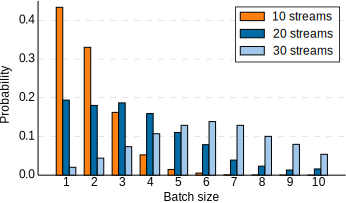
\includegraphics[width=0.6\textwidth]{deepspeech2/figures/batching.pdf}
\caption{Probability that a request is processed in a batch of given size}
\label{fig:deepspeech2:batching}
\end{figure}

In order to deploy our relatively large deep neural networks at low latency, we
have paid special attention to efficiency during deployment. Most internet
applications process requests individually as they arrive in the data center.
This makes for a straightforward implementation where each request can be
managed by one thread. However, processing requests individually is inefficient
computationally, for two main reasons. Firstly, when processing requests
individually, the processor must load all the weights of the network for each
request. This lowers the arithmetic intensity of the workload, and tends to
make the computation memory bandwidth bound, as it is difficult to effectively
use on-chip caches when requests are presented individually. Secondly, the
amount of parallelism that can be exploited to classify one request is limited,
making it difficult to exploit SIMD or multi-core parallelism. RNNs are
especially challenging to deploy because evaluating RNNs sample by sample
relies on sequential matrix vector multiplications, which are bandwidth bound
and difficult to parallelize.

To overcome these issues, we built a batching scheduler called Batch Dispatch
that assembles streams of data from user requests into batches before
performing forward propagation on these batches. In this case, there is a
tradeoff between increased batch size, and consequently improved efficiency,
and increased latency. The more we buffer user requests to assemble a large
batch, the longer users must wait for their results. This places constraints on
the amount of batching we can perform.

We use an eager batching scheme that processes each batch as soon as the
previous batch is completed, regardless of how much work is ready by that
point. This scheduling algorithm has proved to be the best at reducing end-user
latency, despite the fact that it is less efficient computationally, since it
does not attempt to maximize batch size.

Figure~\ref{fig:deepspeech2:batching} shows the probability that a request is
processed in a batch of given size for our production system running on a
single NVIDIA Quadro K1200 GPU, with 10-30 concurrent user requests. As
expected, batching works best when the server is heavily loaded: as load
increases, the distribution shifts to favor processing requests in larger
batches. However, even with a light load of only 10 concurrent user requests,
our system performs more than half the work in batches with at least 2 samples.

\begin{figure}[h]
\centering
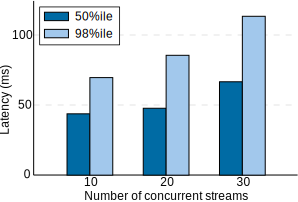
\includegraphics[width=0.6\textwidth]{deepspeech2/figures/latency.pdf}
\caption{Median and 98th percentile latencies as a function of server load}
\label{fig:deepspeech2:latency}
\end{figure}

We see in Figure~\ref{fig:deepspeech2:latency}, that our system achieves a
median latency of 44 ms, and a 98 percentile latency of 70 ms when loaded with
10 concurrent streams. As the load increases on the server, the batching
scheduler shifts work to more efficient batches, which keeps latency low. This
shows that Batch Dispatch makes it possible to deploy these large models at
high throughput and low latency.

\subsection{Deployment Optimized Matrix Multiply Kernels}

We have found that deploying our models using half-precision (16-bit)
floating-point arithmetic does not measurably change recognition accuracy.
Because deployment does not require any updates to the network weights, it is
far less sensitive to numerical precision than training. Using half-precision
arithmetic saves memory space and bandwidth, which is especially useful for
deployment, since RNN evaluation is dominated by the cost of caching and
streaming the weight matrices.

The batch size during deployment is much smaller than in training. We found
that standard BLAS libraries are inefficient at this batch size. To overcome
this, we wrote our own half-precision matrix-matrix multiply kernel. For 10
simultaneous streams over 90 percent of batches are for $N \leq 4$, a regime
where the matrix multiply will be bandwidth bound.  We store the $A$ matrix
transposed to maximize bandwidth by using the widest possible vector loads
while avoiding transposition after loading.  Each warp computes four rows of
output for all $N$ output columns.  Note that for $N \leq 4$ the $B$ matrix
fits entirely in the L1 cache.  This scheme achieves 90 percent of peak
bandwidth for $N \leq 4$ but starts to lose efficiency for larger $N$ as the
$B$ matrix stops fitting into the L1 cache.  Nonetheless, it continues to
provide improved performance over existing libraries up to $N=10$.

\begin{figure}
\centering
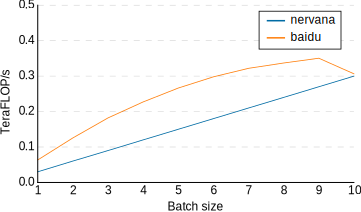
\includegraphics[width=0.6\textwidth]{deepspeech2/figures/hgemm.pdf}
    \caption{Comparison of kernels that compute $A x = b$ where $A$ is a matrix
    with dimension $2560 \times 2560$, and $x$ is a matrix with dimension $2560
    \times \textrm{Batch size}$, where $\textrm{Batch size} \in [1, 10]$. All
    matrices are in half-precision format.}
\label{fig:deepspeech2:hgemm}
\end{figure}

Figure~\ref{fig:deepspeech2:hgemm} shows that our deployment kernel sustains a higher
computational throughput than those from Nervana Systems~\cite{nervana2015} on
the K1200 GPU, across the entire range of batch sizes that we use in
deployment. Both our kernels and the Nervana kernels are significantly faster
than NVIDIA CUBLAS version 7.0, more details are found here~\cite{elsen2015}.

\subsection{Beam Search}

Performing the beam search involves repeated lookups in the \emph{n}-gram
language model, most of which translate to uncached reads from memory. The
direct implementation of beam search means that each time-step dispatches one
lookup per character for each beam. In Mandarin, this results in over 1M
lookups per 40ms stride of speech data, which is too slow for deployment. To
deal with this problem, we use a heuristic to further prune the beam search.
Rather than considering all characters as viable additions to the beam, we only
consider the fewest number of characters whose cumulative probability is at
least $p$. In practice, we have found that $p=0.99$ works well. Additionally,
we limit ourselves to no more than 40 characters. This speeds up the Mandarin
language model lookup time by a factor of 150x, and has a negligible effect on
the CER (0.1-0.3\% relative).

\subsection{Results}

We can deploy our system at low latency and high throughput without sacrificing
much accuracy. On a held-out set of 2000 utterances, our research system
achieves 5.81 character error rate whereas the deployed system achieves 6.10
character error rate. This is only a 5\% relative degradation for the deployed
system. In order to accomplish this, we employ a neural network architecture
with low deployment latency, reduce the precision of our network to 16-bit,
built a batching scheduler to more efficiently evaluate RNNs, and find a simple
heuristic to reduce beam search cost. The model has five forward-only recurrent
layers with 2560 hidden units, one row convolution layer
(Section~\ref{sec:deepspeech2:fom}) with $\tau=19$, and one fully-connected
layer with 2560 hidden units. These techniques allow us to deploy Deep Speech
at low cost to interactive applications.
